\documentclass[a4paper]{article}
\usepackage[left=2.1cm, right=2.1cm, top=2.1cm]{geometry}
\usepackage{lipsum}
\usepackage{tikzpagenodes}
\usepackage{pgfplots}
\usepackage{tikz}
\usepackage{tikz-3dplot}
\usetikzlibrary{arrows,decorations.pathmorphing,backgrounds,positioning,fit,matrix}
\pgfplotsset{compat=1.8}
\usepackage{graphics} % for pdf, bitmapped graphics files
\usepackage{epsfig} % for postscript graphics files
\usepackage[colorlinks=true,citecolor=green]{hyperref}
\usepackage{cite}
\usepackage{amsmath,amssymb,amsfonts}
\usepackage{algorithmic}
\usepackage{graphicx}
\usepackage{url}
\usepackage{cite}
\usepackage{bm}
\usepackage{pbox}
\usepackage{siunitx,booktabs,etoolbox}
\usepackage{ulem}
\usepackage[framed,numbered,autolinebreaks,useliterate]{mcode}
\usepackage{filecontents}
%\usepackage{bigfoot} % to allow verbatim in footnote


\def\BibTeX{{\rm B\kern-.05em{\sc i\kern-.025em b}\kern-.08em
    T\kern-.1667em\lower.7ex\hbox{E}\kern-.125emX}}


\begin{document}

\title{Exercise on Fast feature detector, brief descriptor \& feature matching}
\author{xiahaa@space.dtu.dk}
\maketitle%%

In this exercise, you will work on Fast corner detector, Brief descriptor as we as brute-force based feature matching.

\section{Fast Feature Detector}
\begin{enumerate}
\item Generate Fast template (A bresenham circle with $16$ pixels).
\item Traverse the whole image, compare the center pixel with the neighboring pixels in the template. If $|I_{nn}-I_{c}| \geq t$, it counts $1$, otherwise $0$. Check if there are $12$ contiguous pixels being $1$, then this is a corner.
\item Apply nonmaxima suppression.
\end{enumerate}

\textbf{It is a good idea to organize your code as separate functions which can be reused.}

\begin{figure*}[!b]
\centering
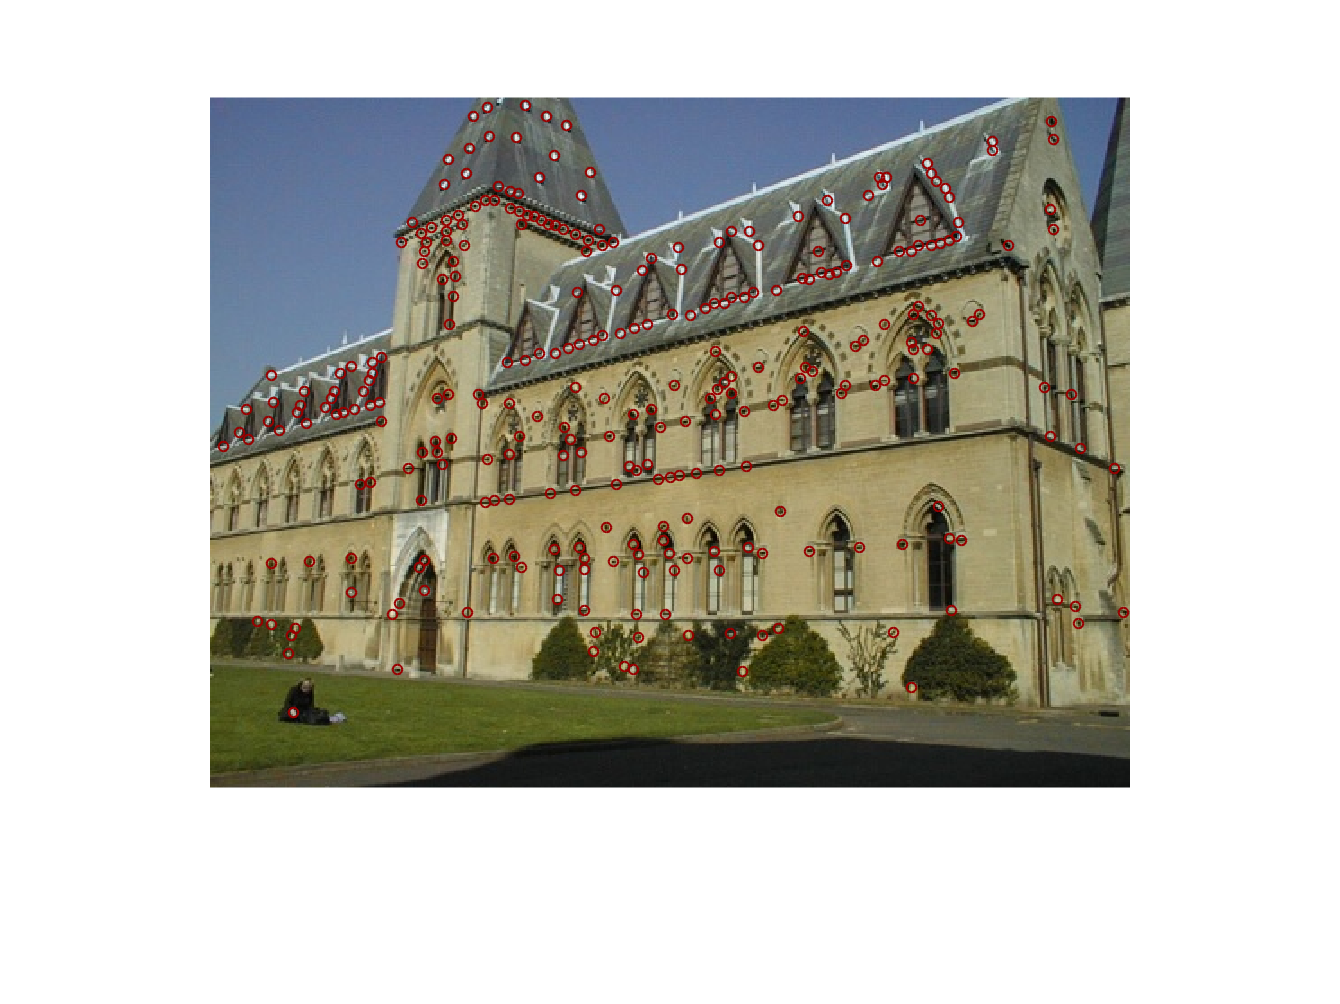
\includegraphics[scale=0.3]{figures/fastc.png}
\caption{Example of Fast detection result.}
\end{figure*}


\section{Brief Feature Descriptor}
\begin{enumerate}
	\item Generate Brief pattern (you can use the one I upload) which looks like Figure~\ref{fig:bb}. This pattern is an array of pairs. For example, if we want to generate a Brief pattern of $128$ bits, then the pattern is nothing but a array of $\mathbf{A}_{4 \times 128}$ with each column being the coordinates of two points to compare, e.g.  $\mathbf{A}(:, 1)=[1, 1, 3, -4]^T$ which means we for the fist bit, we would like to compare the intensity of the neighboring pixel $(i+1,j+1)$ and pixel $(i+3,j-4)$. 
	\item load pattern and apply the test for all comparison pairs, concatenate them as a vector. Suppose you are using $128$ bits and you have $n$ features, then you will get an array of $n \times 128$ with each row being a descriptor for one corner.
\end{enumerate}
\begin{figure*}[!b]
	\centering
	\label{fig:bb}
	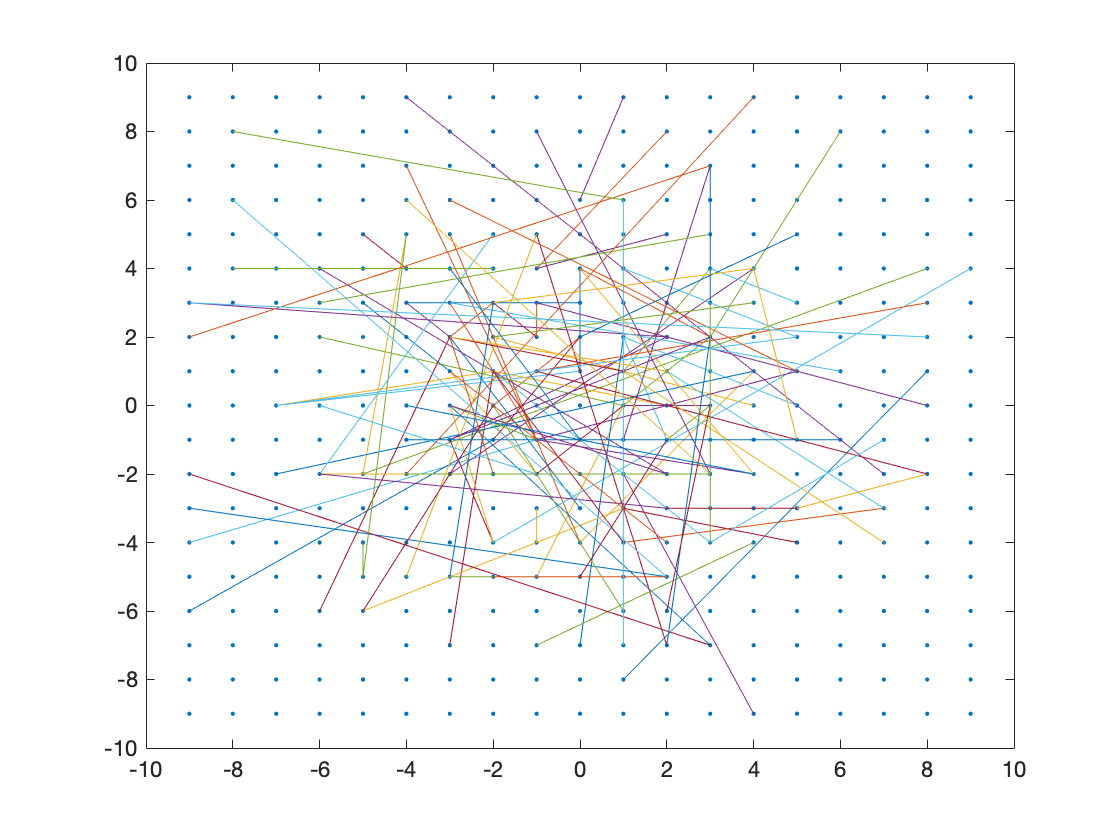
\includegraphics[scale=0.3]{figures/brief_pattern.png}
	\caption{Example of Brief pattern.}
\end{figure*}

\section{Feature matching}
With feature descriptor, feature matching can be done as follows:
 \begin{enumerate}
 	\item for each feature in image $i$, use its descriptor $d_i$ to compare all the descriptors in image $j, j=1,2,\cdots,n$, compute the so called Hamming distance which is sum of the $XOR$ result. For example, the vectors shown in the above figure have a Hamming distance of $4$.
 	\item choose the one with the minimum distance as the matched feature point.
 	\item do this for all feature points.
 \end{enumerate}
 \begin{table}
 	\begin{tabular}{|c|c|c|c|c|c|c|c|}
 		\hline
 	{1} & {0} & {1} & {0} & {1} & {0} & {1} & {1} \\
 		\hline
 \end{tabular} \newline
 	\begin{tabular}{cccccccccc}
	{ } & { } & { } & { } & { } & { } & { } & { } & { } &{$\searrow$} \\
	 \end{tabular} \newline
  	\begin{tabular}{ccccccccccc|c|c|c|c|c|c|c|c|}
 	{ } & { } & { } & { } & { } & { } & { } & { } & { } &{} & { } & {1} & {1} & {0} & {0} & {0} & {1} & {1} &{0} 
 \end{tabular} \newline
  	\begin{tabular}{cccccccccc}
 	{ } & { } & { } & { } & { } & { } & { } & { } & { } &{$\nearrow$} \\
 \end{tabular} \newline
\begin{tabular}{|c|c|c|c|c|c|c|c|}
	\hline
	 	0                     & 1                     & 1                     & 0                     & 1                     & 1                     & 0                     & 1    \\
	 	\hline
\end{tabular} 
 \end{table}
%\bibliography{hand_eye_calibration} 
%\bibliographystyle{ieeetr}
\begin{figure*}[!b]
	\centering
	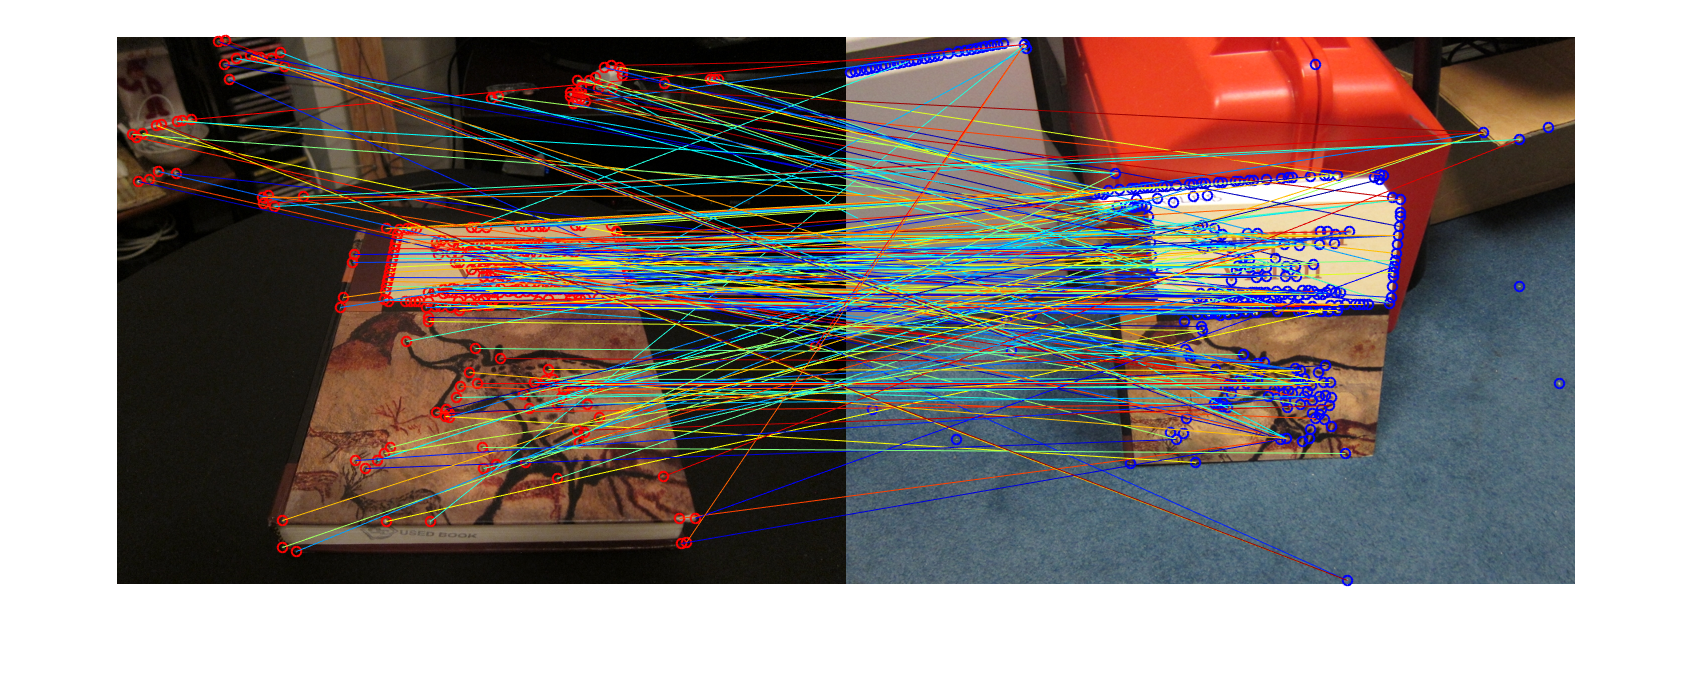
\includegraphics[scale=0.3]{figures/fast.png}
	\caption{Example of feature matching result.}
\end{figure*}
\end{document}